%%
%% This is file `sample-manuscript.tex',
%% generated with the docstrip utility.
%%
%% The original source files were:
%%
%% samples.dtx  (with options: `manuscript')
%%
%% IMPORTANT NOTICE:
%%
%% For the copyright see the source file.
%%
%% Any modified versions of this file must be renamed
%% with new filenames distinct from sample-manuscript.tex.
%%
%% For distribution of the original source see the terms
%% for copying and modification in the file samples.dtx.
%%
%% This generated file may be distributed as long as the
%% original source files, as listed above, are part of the
%% same distribution. (The sources need not necessarily be
%% in the same archive or directory.)
%%
%% Commands for TeXCount
%TC:macro \cite [option:text,text]
%TC:macro \citep [option:text,text]
%TC:macro \citet [option:text,text]
%TC:envir table 0 1
%TC:envir table* 0 1
%TC:envir tabular [ignore] word
%TC:envir displaymath 0 word
%TC:envir math 0 word
%TC:envir comment 0 0
%%
%%
%% The first command in your LaTeX source must be the \documentclass command.
%%%% Small single column format, used for CIE, CSUR, DTRAP, JACM, JDIQ, JEA, JERIC, JETC, PACMCGIT, TAAS, TACCESS, TACO, TALG, TALLIP (formerly TALIP), TCPS, TDSCI, TEAC, TECS, TELO, THRI, TIIS, TIOT, TISSEC, TIST, TKDD, TMIS, TOCE, TOCHI, TOCL, TOCS, TOCT, TODAES, TODS, TOIS, TOIT, TOMACS, TOMM (formerly TOMCCAP), TOMPECS, TOMS, TOPC, TOPLAS, TOPS, TOS, TOSEM, TOSN, TQC, TRETS, TSAS, TSC, TSLP, TWEB.
% \documentclass[acmsmall]{acmart}

%%%% Large single column format, used for IMWUT, JOCCH, PACMPL, POMACS, TAP, PACMHCI
% \documentclass[acmlarge,screen]{acmart}

%%%% Large double column format, used for TOG
% \documentclass[acmtog, authorversion]{acmart}

%%%% Generic manuscript mode, required for submission
%%%% and peer review
\documentclass[review, sigplan]{acmart}
\usepackage{listings}
\usepackage{amsmath}
\settopmatter{printacmref=false,printccs=false}
\renewcommand\footnotetextcopyrightpermission[1]{} % removes footnote with conference information in first column

%% Fonts used in the template cannot be substituted; margin
%% adjustments are not allowed.
%%
%% \BibTeX command to typeset BibTeX logo in the docs
%\AtBeginDocument{%
%  \providecommand\BibTeX{{%
%    \normalfont B\kern-0.5em{\scshape i\kern-0.25em b}\kern-0.8em\TeX}}}

%% Rights management information.  This information is sent to you
%% when you complete the rights form.  These commands have SAMPLE
%% values in them; it is your responsibility as an author to replace
%% the commands and values with those provided to you when you
%% complete the rights form.
%\setcopyright{acmcopyright}
%\copyrightyear{2018}
%\acmYear{2018}
%\acmDOI{XXXXXXX.XXXXXXX}

%% These commands are for a PROCEEDINGS abstract or paper.
%\acmConference[Conference acronym 'XX]{Make sure to enter the correct
%  conference title from your rights confirmation emai}{June 03--05,
%  2018}{Woodstock, NY}
%
%  Uncomment \acmBooktitle if th title of the proceedings is different
%  from ``Proceedings of ...''!
%
%\acmBooktitle{Woodstock '18: ACM Symposium on Neural Gaze Detection,
% June 03--05, 2018, Woodstock, NY}
%\acmPrice{15.00}
%\acmISBN{978-1-4503-XXXX-X/18/06}


%%
%% Submission ID.
%% Use this when submitting an article to a sponsored event. You'll
%% receive a unique submission ID from the organizers
%% of the event, and this ID should be used as the parameter to this command.
%%\acmSubmissionID{123-A56-BU3}

%%
%% For managing citations, it is recommended to use bibliography
%% files in BibTeX format.
%%
%% You can then either use BibTeX with the ACM-Reference-Format style,
%% or BibLaTeX with the acmnumeric or acmauthoryear sytles, that include
%% support for advanced citation of software artefact from the
%% biblatex-software package, also separately available on CTAN.
%%
%% Look at the sample-*-biblatex.tex files for templates showcasing
%% the biblatex styles.
%%

%%
%% The majority of ACM publications use numbered citations and
%% references.  The command \citestyle{authoryear} switches to the
%% "author year" style.
%%
%% If you are preparing content for an event
%% sponsored by ACM SIGGRAPH, you must use the "author year" style of
%% citations and references.
%% Uncommenting
%% the next command will enable that style.
%%\citestyle{acmauthoryear}

\lstset{mathescape, basicstyle=\ttfamily}
%%
%% end of the preamble, start of the body of the document source.
\begin{document}

%%
%% The "title" command has an optional parameter,
%% allowing the author to define a "short title" to be used in page headers.
\title{Cobb: Synthesis of Test Input Generators with Coverage Types}

%%
%% The "author" command and its associated commands are used to define
%% the authors and their affiliations.
%% Of note is the shared affiliation of the first two authors, and the
%% "authornote" and "authornotemark" commands
%% used to denote shared contribution to the research.
\author{Patrick LaFontaine}
\author{Anxhelo Xhebraj}
\author{David Deng}
%\email{}
%\affiliation{%
%    \institution{Purdue University}
%    \streetaddress{}
%    \city{}
%    \state{}
%    \country{USA}
%    \postcode{}
%}


%%
%% By default, the full list of authors will be used in the page
%% headers. Often, this list is too long, and will overlap
%% other information printed in the page headers. This command allows
%% the author to define a more concise list
%% of authors' names for this purpose.
\renewcommand{\shortauthors}{LaFontaine et al.}


%\begin{abstract}
%    This thing is cool
%\end{abstract}

%%
%% The code below is generated by the tool at http://dl.acm.org/ccs.cfm.
%% Please copy and paste the code instead of the example below.
%%
%\begin{CCSXML}

%\end{CCSXML}



%%
%% Keywords. The author(s) should pick words that accurately describe
%% the work being presented. Separate the keywords with commas.
%\keywords{Do, Not, Us, This, Code, Put, the, Correct, Terms, for, Your, Paper}


%\received{20 February 2007}
%\received[revised]{12 March 2009}
%\received[accepted]{5 June 2009}

%%
%% This command processes the author and affiliation and title
%% information and builds the first part of the formatted document.
\maketitle


\section*{What we've done so far}

\begin{itemize}
    \item Setup project structure
          \begin{itemize}
              \item Gather all libraries needed
              \item Set up a runnable project that can use said libraries
          \end{itemize}
    \item Familiarize ourselves with the Poirot code base
    \item Understand and implement component discovery
          \begin{itemize}
              \item Understand various intermediate representations
              \item Figure out how global configuration is setup: library versus primitive operations, base and coverage type
              signatures, other global mutable state
          \end{itemize}
    \item Step through under-approximate type inference and checking, found out that A-normal form is used, multiple contexts and symbol lookup.
    \item Designed an incremental and fused type inference/ synthesis engine by raising subexpression into the typing context to avoid redundant work
          \begin{itemize}
              \item In bottom-up synthesis, a program is typically extended by constructing a new root node to combine child AST's. In nested A-normal form, extending a program requires substituting the innermost body with the new root expression.
              \item Additionally, type inference would need to traverse the same sub-expressions every time that expression is leveraged in a new larger expression.
              \item Our solution is to represent sub-expressions by their variable bindings in the typing context with a side mapping to reconstruct terms. Synthesis of a new term is then the merging of typing contexts and the construction of an application of the component on the argument names.
          \end{itemize}
    \item We abstract over the implementations of the various operation and value kinds into two synthesis abstractions: seeds and components.
          \begin{itemize}
              \item Seed terms provide the starting point of our enumeration as our leaf nodes and are made up of our argumentless constructors like \texttt{Nil}, thunked operations like generators, constant values( like \texttt{0}, \texttt{1}, \texttt{true}, \texttt{false}), and variables as introduced as arguments by the function signature.
              \item Components are our abstraction over the ways to construct new terms using primitive operations like \texttt{==}, built-in library functions like \texttt{Cons}, user-provided functions like \texttt{int\_range\_inc}, and the recursive call. Note that the recursive call gains an additional constraint requiring the first argument to be smaller than the first argument in the context. Each component has a generalized apply operation to construct a new term.
          \end{itemize}
    \item Thus we introduced our notion of blocks, program expressions without control flow.
          \begin{itemize}
              \item Leveraging the above abstractions and typing contexts,
                    our enumeration constructs blocks which contain a binding name,
                    an associated typing context, and a simple term which may
                    reference variables in said typing context.
              \item Each of these blocks are stored in a mapping from a base type
                    to list of blocks which represent the enumerated blocks of
                    said type.
                    We initialize this map with our seeds at the beginning of synthesis.
              \item At each step, we separate the blocks into two kinds, those
                    of the largest depth which is equivalent to the number of times
                    we have iterated so far and all of the smaller terms.
                    The blocks of the largest depth are relevant as each new term we
                    construct must reference at least one of these blocks.
                    This guarantees incremental growth of our blocks and avoids constructing redundant terms.
              \item After each step, we currently only do a naive extraction of the
                    final program.
                    If a block is a valid subtype of our target, then we extract out
                    the term of that block and return.
                    If there is no obvious candidate, we perform a cross product of
                    all blocks using non-deterministic choice which we construct as
                    an if expression using \texttt{bool\_gen} as the condition.
                    If that also fails to produce a satisfying term then we
                    recurse to construct blocks fo the next depth.
          \end{itemize}

\end{itemize}


\section*{What we plan to do}

\begin{enumerate}
    \item \textbf{Block join exploration}
    Currently we pairwise combine blocks with control-flow
    without prioritization.
    It would be ideal if we can ensure that the combined
    blocks increase coverage to reduce exploration.
    \item \textbf{Improve extractions} Currently our strategy returns any program that satisfies
    the signature provided.
    Given the exploration strategy, this produces the smallest
    program that satisfies the specification.
    However, especially in the context of under-approximate
    types, it might be beneficial to explore further to
    synthesize a program that is safer (generates less spurious
    test cases that don't meet the over-approximate version of
    the specification).
    \item \textbf{Specializing generators}
    A key issue of the current synthesis approach is that
    the addition of control-flow is only through
    non-determinstic choice \\ \lstinline{if bool_gen() then $\square$ else $\square$}.
    Instead, it could be more beneficial to add control-flow
    that depends on arguments or other subterms such as
    \texttt{if is\_nil(arg1)}.
    Moreover, to reduce the search space, use of subterms
    are not shared. Consider the image below

    \begin{figure}[h!]
    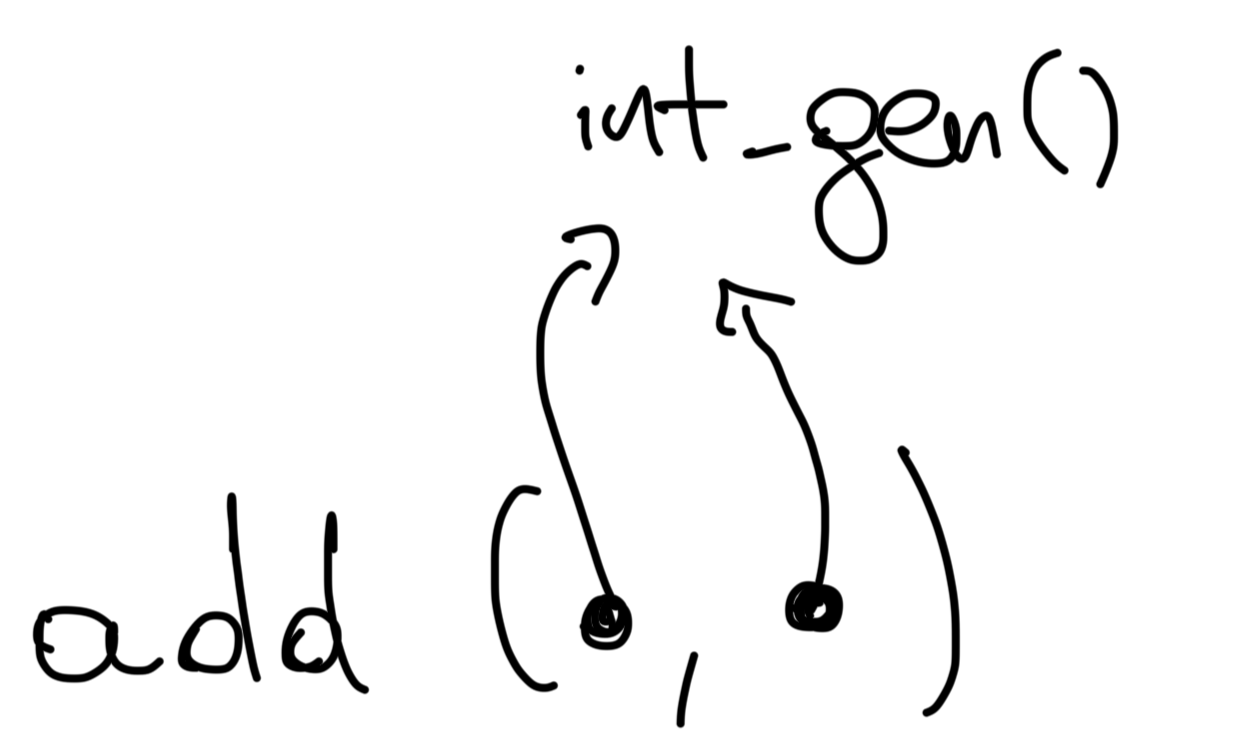
\includegraphics[width=.2\textwidth]{img.png}
    \end{figure}

    there are two possible program interpretations
    \begin{enumerate}
        \item \texttt{let x = int\_gen(); add(x, x)}
        \item \texttt{add(int\_gen(), int\_gen())}
    \end{enumerate}
    we currently opt for the latter one (b) which is
    complete but possibly unsafe.
    For example, if the under-approximate specification was
    ${\textcolor{blue}[}\nu : \textsf{int} \mid \textsf{even}(\nu){\textcolor{blue}]}$,
    program (a) would also satisfy the over-approximate type
    ${\textcolor{red}\{}\nu : \textsf{int} \mid \textsf{even}(\nu){\textcolor{red}\}}$
    while (b) wouldn't.
    % a non-deterministic expression might be subsuming a
    % deterministic expression.
\end{enumerate}

\section*{How will we accomplish that plan}

% let x = int_gen()
% let y = int_gen()
% add(x, y)

\begin{enumerate}
\item \textbf{Block join exploration}
    We can perform pairwise subtype checks to avoid
    combining blocks that do not increase coverage.

\item \textbf{Improve extractions}
    We can infer the \emph{over}-approximate
    specifications of the potential candidates and rule
    out candidates that are supertypes of other candidates.
    Additionally we can run the candidates and select the
    ones that statistically produce results that
    meet the under-approximate type.

\item \textbf{Specializing generators}
    To fix the control-flow issue we can easily add candidates
    other than non-determinstic choice to discriminate
    over when building conditionals.
    For whether to interpret uses of the same non-deterministic
    subexpressions as by name or by value,
    we can either choose to add the possibility
    of naming sub-expressions (let-bindings) and add
    such names as possible subterms or post-process
    the candidates to reduce non-determinism while maintaining
    coverage.
\end{enumerate}

%%
%% The next two lines define the bibliography style to be used, and
%% the bibliography file.
\bibliographystyle{ACM-Reference-Format}
% \bibliography{cobb}


\end{document}
\endinput
